\section{도메인 정책}
\label{app:domain-policies}

\subsection{검증된 항공 및 소매 정책}

\subsubsection{소매 정책}
\label{app:retail-policy}
\inputminted[escapeinside=||, fontsize=\small, breaklines, breaksymbol=, breaksymbolleft=, breaksymbolright=, breakanywhere, bgcolor=blue!5]{markdown}{codes/retail_agent_policy.md}

\subsubsection{항공 정책}
\label{app:airline-policy}
\inputminted[escapeinside=||, fontsize=\small, breaklines, breaksymbol=, breaksymbolleft=, breaksymbolright=, breakanywhere, bgcolor=green!5]{markdown}{codes/airline_agent_policy.md}

\subsection{통신 정책}
\label{app:telecom-policy}

통신 정책은 두 부분으로 구성된다:
\begin{itemize}
    \item 일반 정책 \Cref{app:generic-telecom-policy}
    \item 기술 지원 정책(기본 및 워크플로) \Cref{app:technical-support-policy,app:technical-support-policy-workflow}
\end{itemize}

\subsubsection{일반 통신 정책}
\label{app:generic-telecom-policy}


\inputminted[escapeinside=||, fontsize=\small, breaklines, breaksymbol=, breaksymbolleft=, breaksymbolright=, breakanywhere, bgcolor=purple!5]{markdown}{codes/telecom_agent_generic.md}

\subsubsection{기술 지원 정책(원본)}
\label{app:technical-support-policy}

\inputminted[escapeinside=||, fontsize=\small, breaklines, breaksymbol=, breaksymbolleft=, breaksymbolright=, breakanywhere, bgcolor=purple!5]{markdown}{codes/telecom_agent_troubleshooting.md}

\solomode 모드에서는, 필요할 때 다시 표현된 이러한 정책들의 버전이 에이전트에게 제공된다.
(예: "ask user to do X"와 같은 지시는 "perform action X"로 다시 표현된다.)


\subsubsection{기술 지원 정책(워크플로)}
\label{app:technical-support-policy-workflow}

\inputminted[escapeinside=||, fontsize=\small, breaklines, breaksymbol=, breaksymbolleft=, breaksymbolright=, breakanywhere, bgcolor=purple!5]{markdown}{codes/telecom_agent_troubleshooting.md}

\subsubsection{문제 해결 워크플로 그래프}
\label{app:troubleshooting-workflow-graphs}

에이전트가 문제 해결 워크플로를 이해하도록 돕기 위해, 각 문제 유형에 대한 의사결정 그래프를 제공한다.

\begin{figure}[htbp]
    \centering
    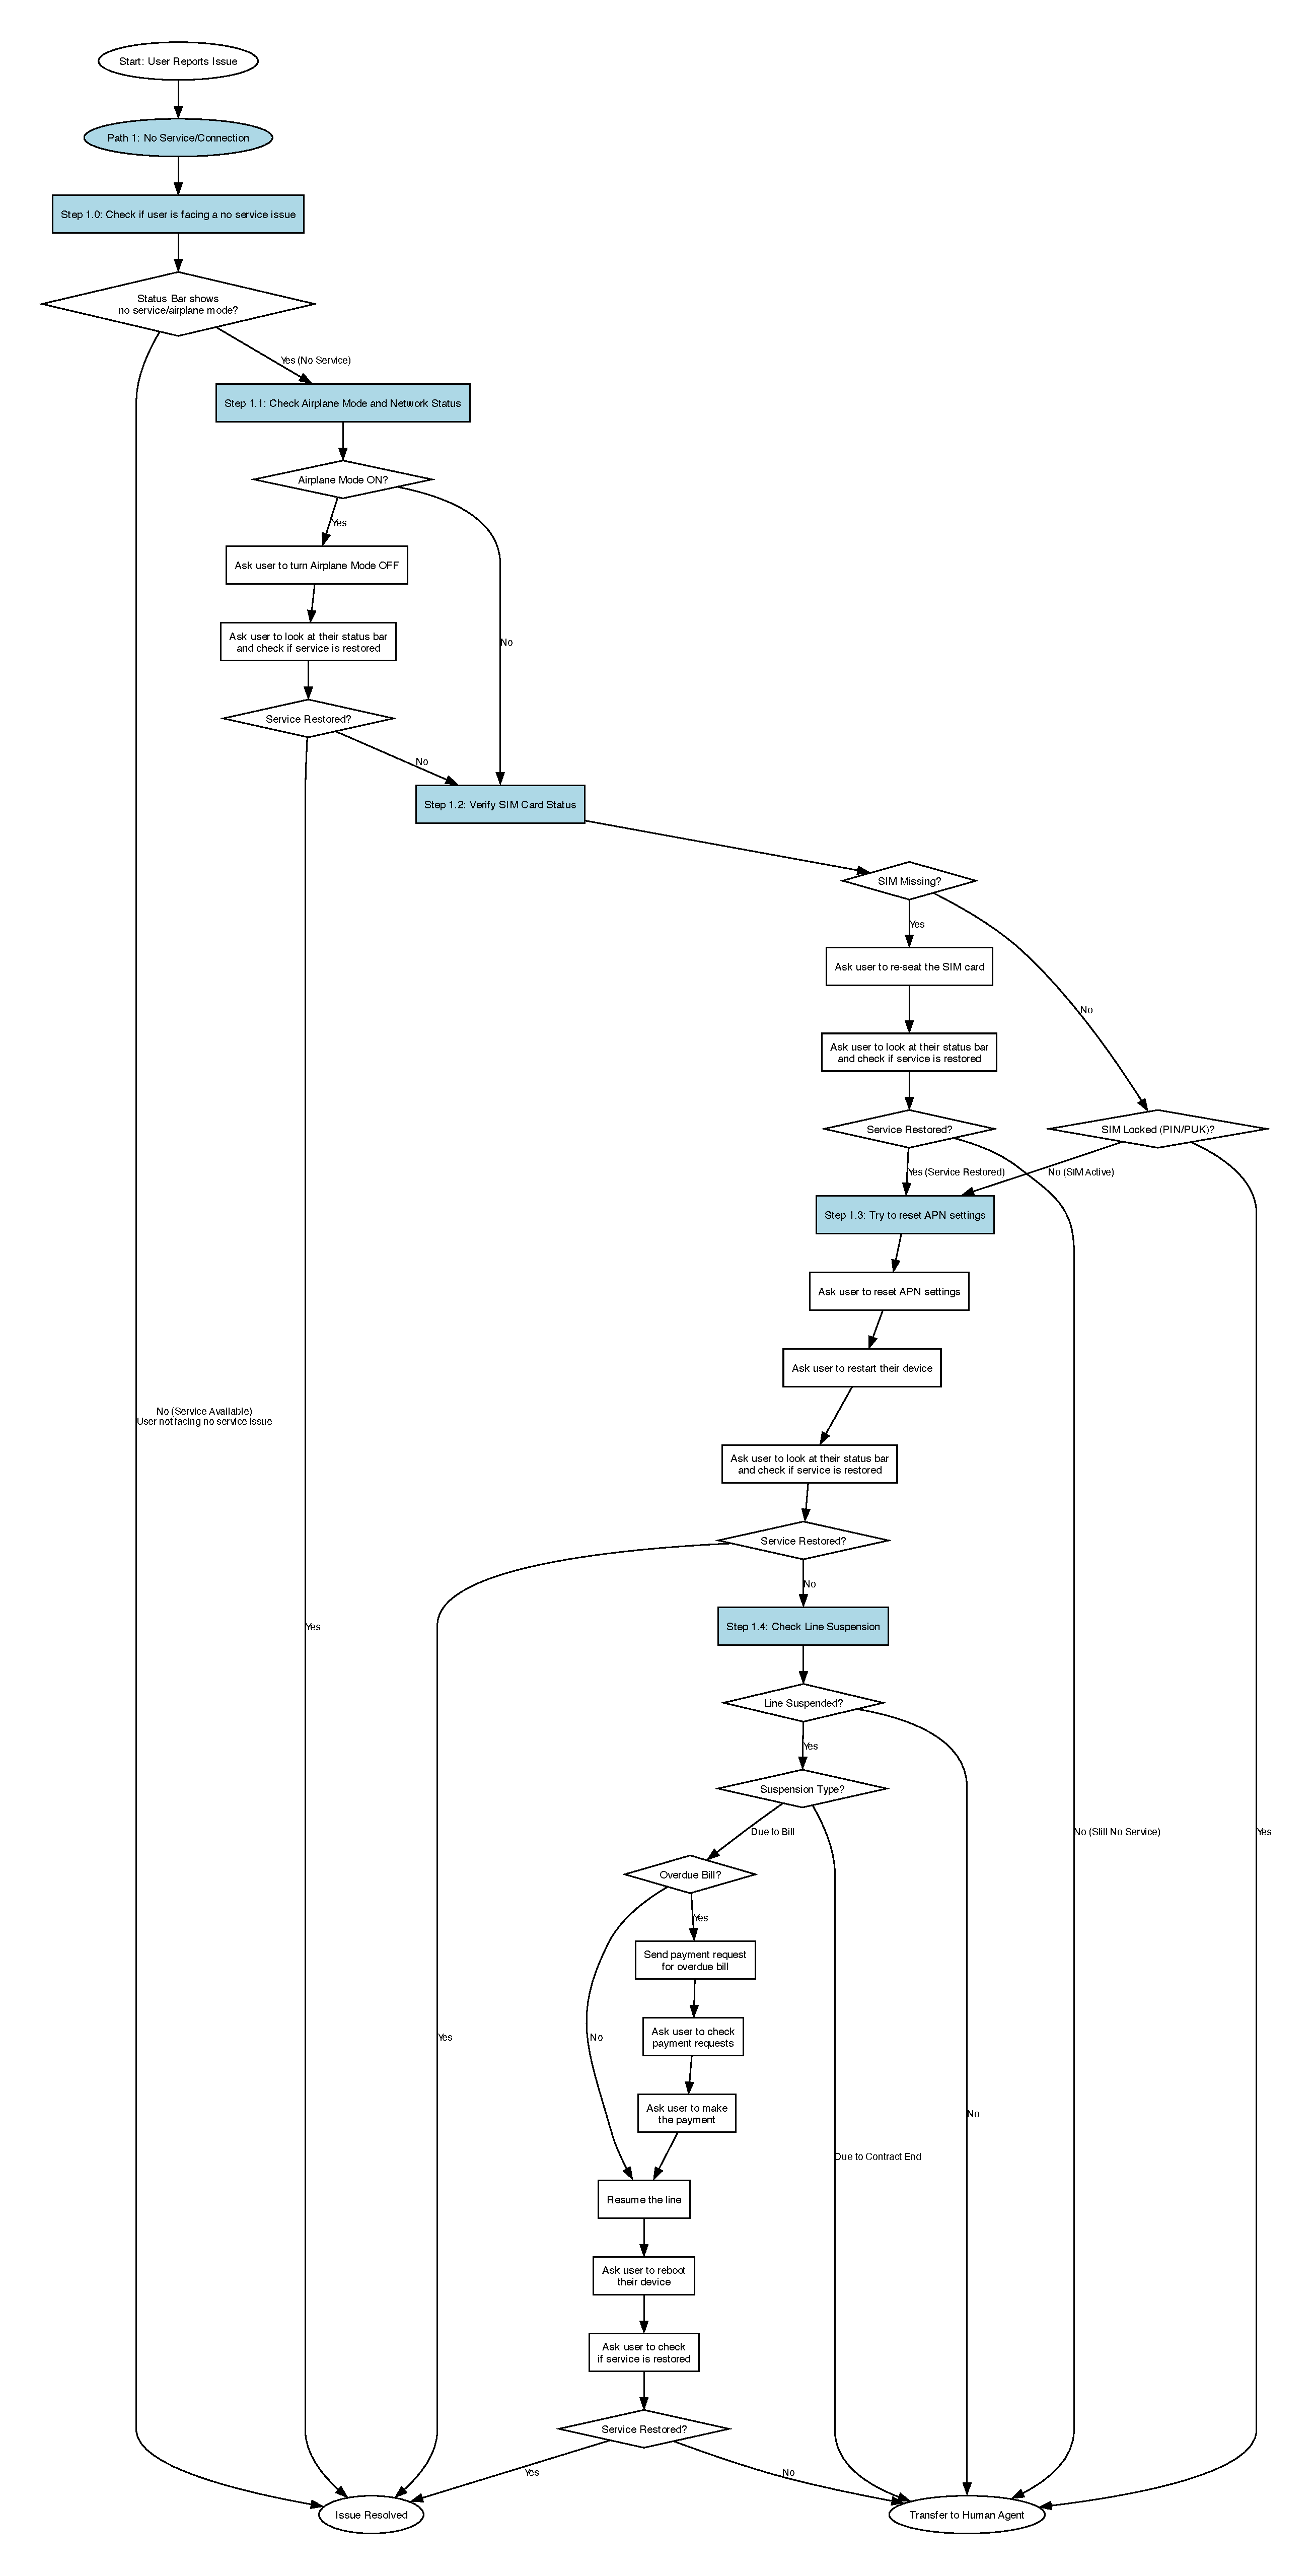
\includegraphics[width=0.7\textwidth]{figures/workflows/tech_support_path1_no_service.pdf}
    \caption{\serviceissue 에 대한 문제 해결 워크플로}
    \label{fig:workflow-no-service}
\end{figure}

\begin{figure}[htbp]
    \centering
    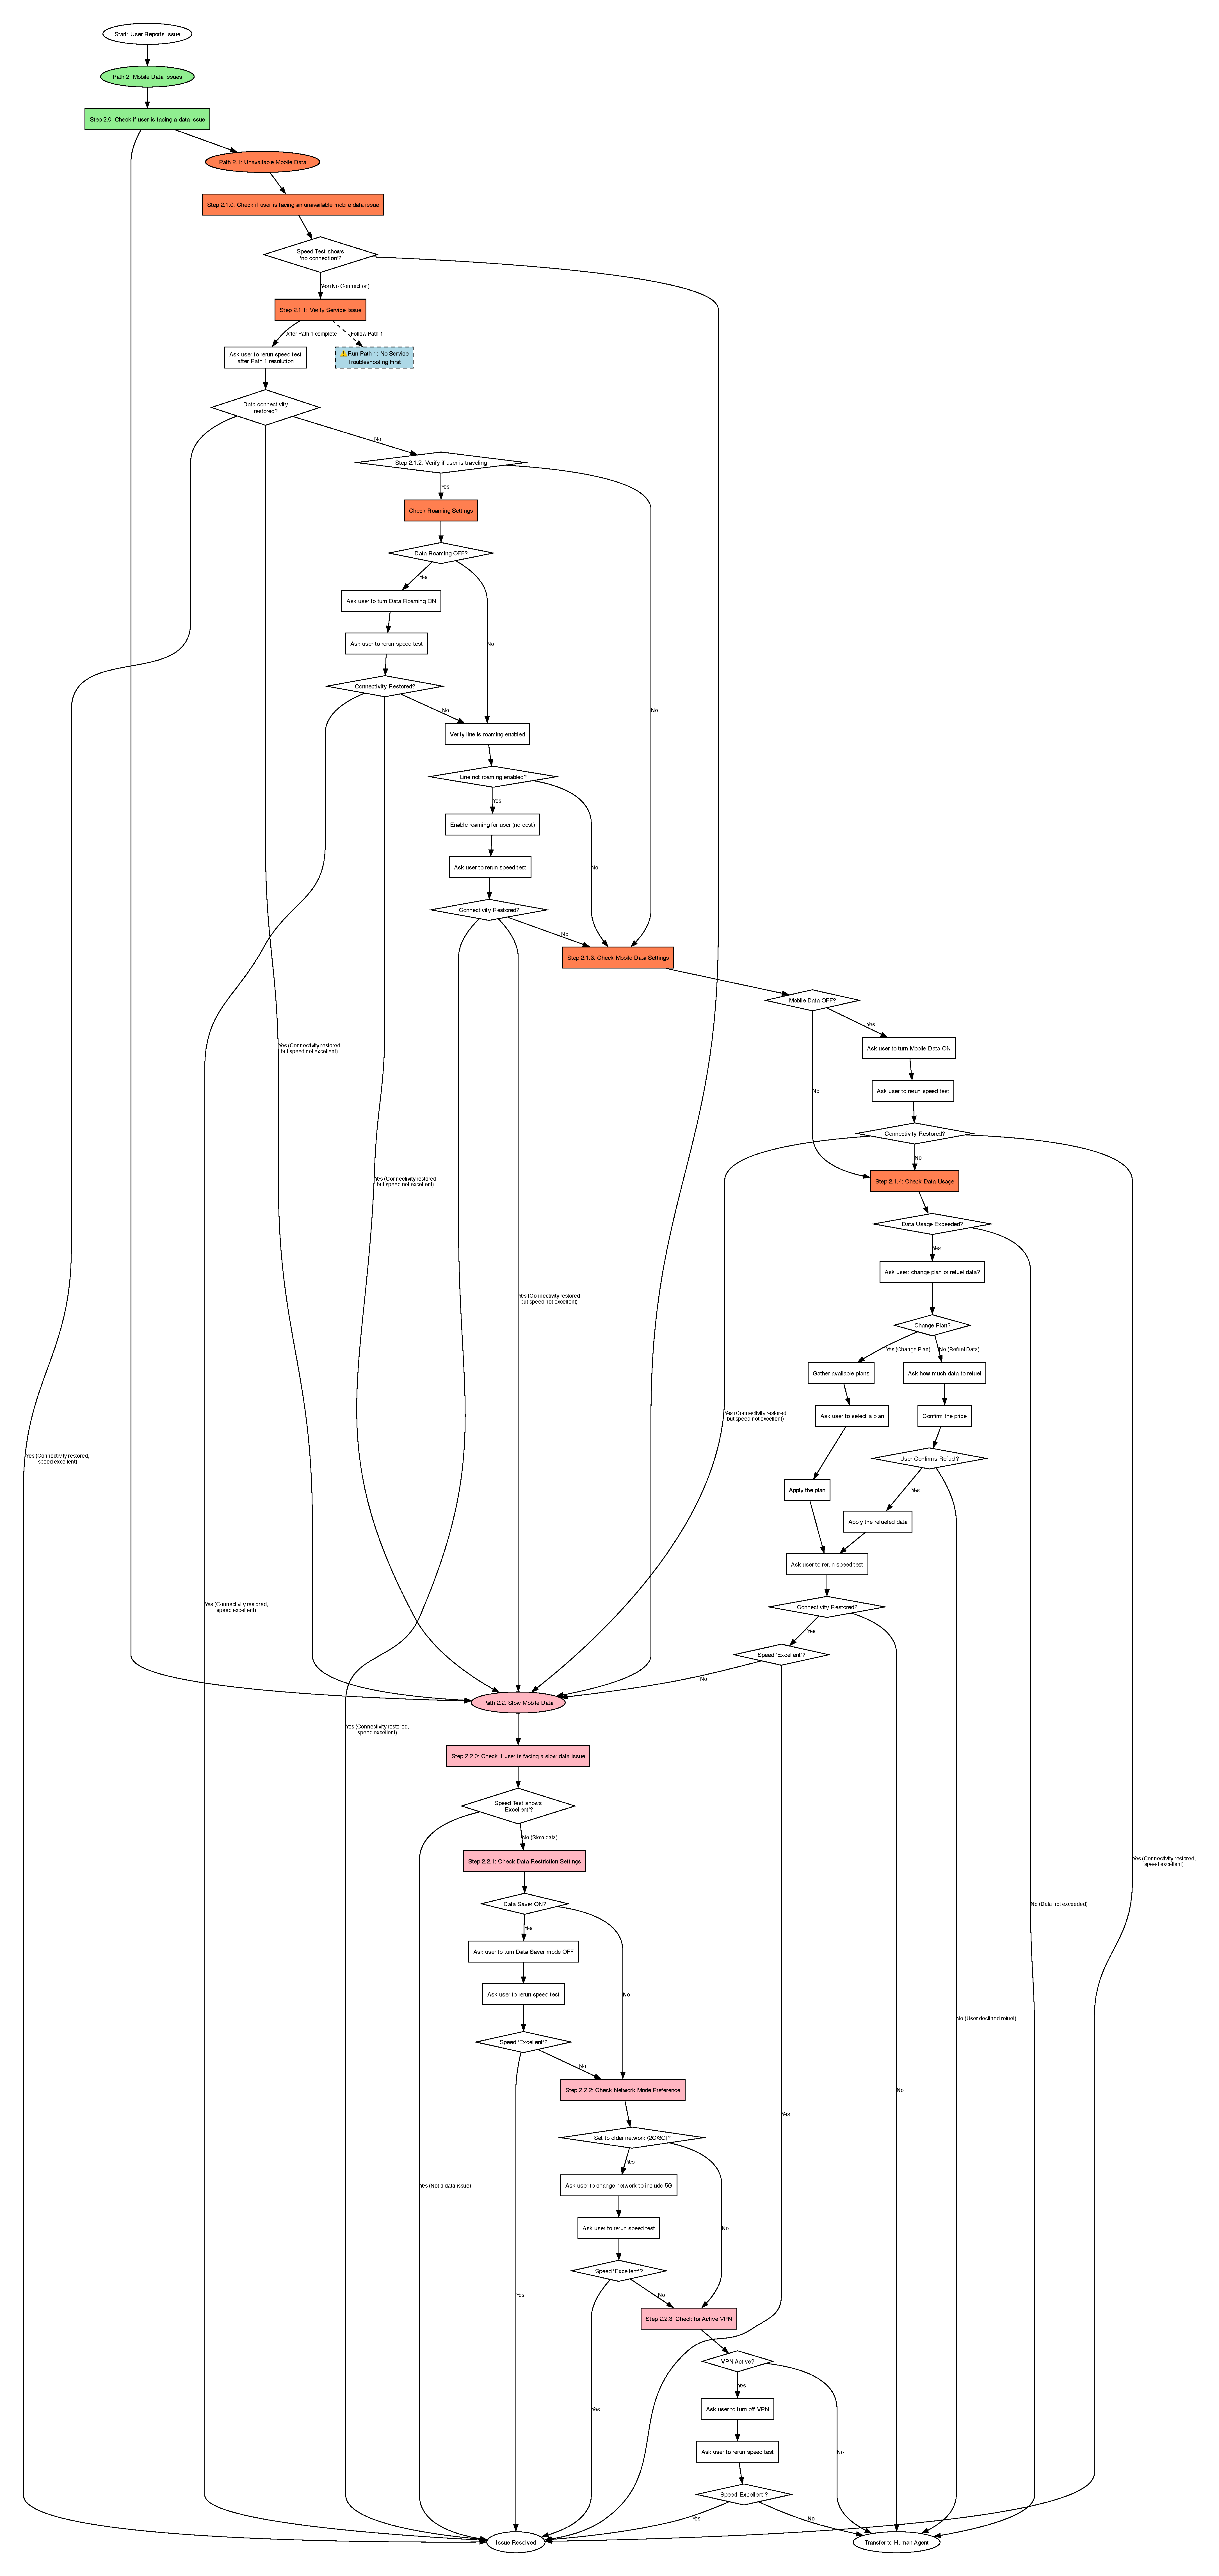
\includegraphics[width=0.7\textwidth]{figures/workflows/tech_support_path2_mobile_data.pdf}
    \caption{\mobiledataissue 에 대한 문제 해결 워크플로}
    \label{fig:workflow-mobile-data}
\end{figure}

\begin{figure}[htbp]
    \centering
    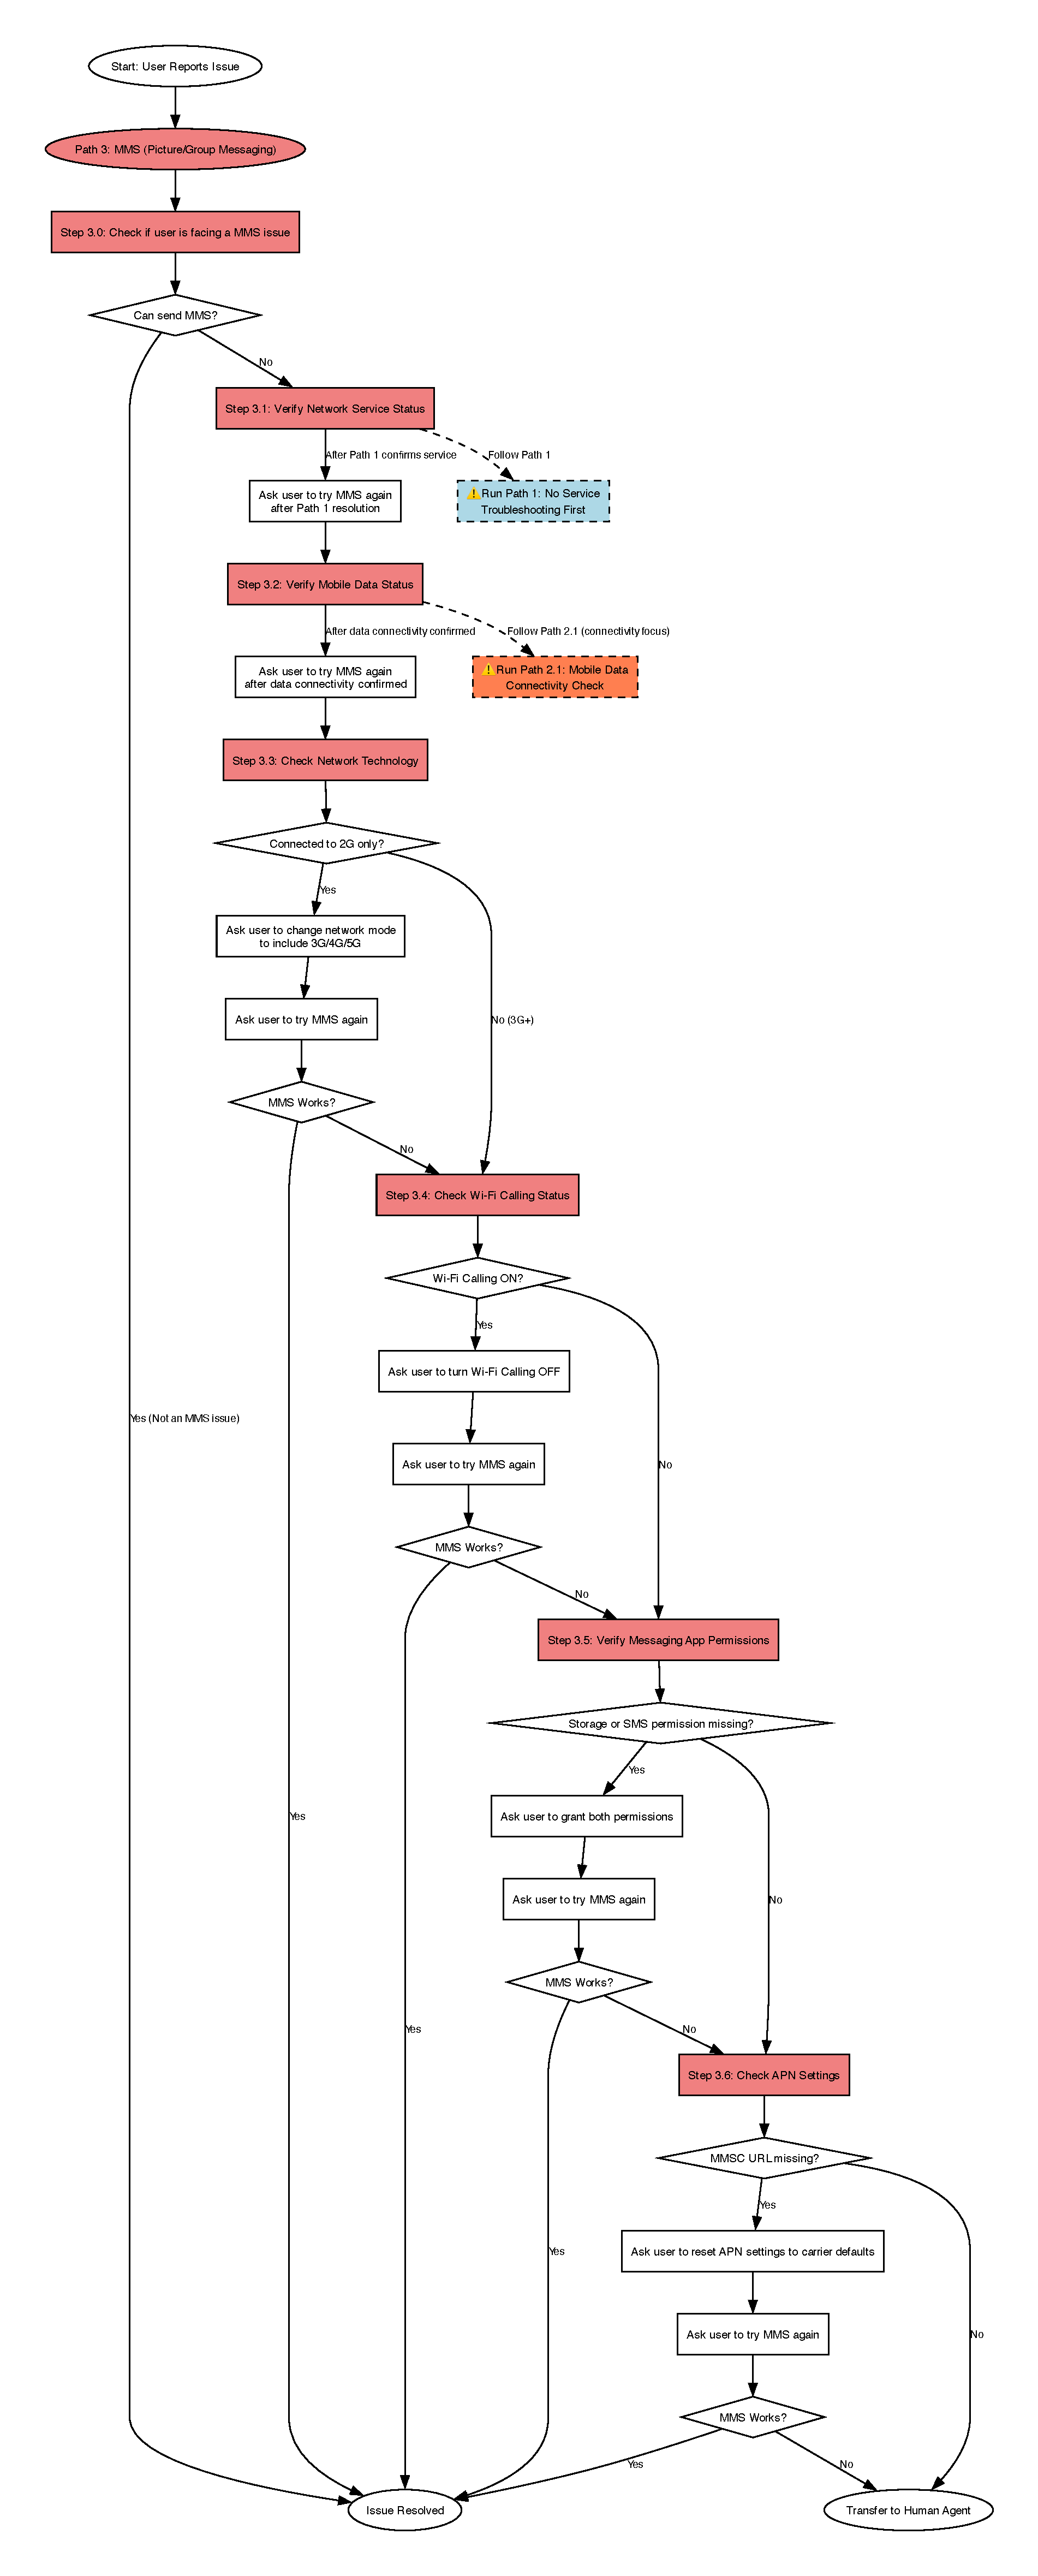
\includegraphics[width=0.7\textwidth]{figures/workflows/tech_support_path3_mms.pdf}
    \caption{\mmsissue 에 대한 문제 해결 워크플로}
    \label{fig:workflow-mms}
\end{figure}
